% TEXTALLION
% https://bitbucket.org/farvardin/textallion
% \LaTeX template 

\documentclass[openany]{book} % openany to remove the blank pages
% use report instead of article so you can use the "chapter"
%\documentclass[oneside]{book}
%\documentclass{article}
%\documentclass[twoside]{article}
%\noitemsep ?
% book = margins are shifted
% article = no shift for margins

\usepackage[activate={true,nocompatibility},final,tracking=true,kerning=true,spacing=true,factor=1100,stretch=10,shrink=10]{microtype}
% activate={true,nocompatibility} - activate protrusion and expansion
% final - enable microtype; use "draft" to disable
% tracking=true, kerning=true, spacing=true - activate these techniques
% factor=1100 - add 10% to the protrusion amount (default is 1000)
% stretch=10, shrink=10 - reduce stretchability/shrinkability (default is 20/20)

\flushbottom
\uchyph=0

\usepackage[pdftex]{graphicx}


\usepackage{paralist} % needed for compact lists
\usepackage[normalem]{ulem} % needed by strike
%  %hyperref defined elsewhere
\usepackage[utf8]{inputenc}  % char encoding
\usepackage{../includes/sample_cyoa}  % user defined

%todo: check this:
\usepackage[protrusion=true,expansion=true]{microtype}


%---------------- Author & Metatags ------------------------------------

\def\DOCUMENTxTITLE{Template} % Titre of the document
\def\PDFAUTHOR{Farvardin}      % Authors
\def\PDFTITLE{\DOCUMENTxTITLE}      % copy of Titre of the document
\def\PDFSUBJECT{cyoa, template, wip, not finished} % Subjet
\def\PDFKEYWORDS{cyoa, template, wip, not finished}   % keywords, tags
\def\PDFCREATOR{Textallion, txt2tags, PdfTeX}   % Sofware which made this document
\def\PDFPRODUCER{Textallion}         % Compagny which made the software

% 

\usepackage[english,frenchb,francais]{babel}  
\usepackage[T1]{tipa}                       % additionnal fonts
\usepackage[\DEFAULTxFONTxSIZE pt]{extsizes} 
\usepackage[cm]{aeguill}                    % French guillemets
\usepackage[\SIZExOFxPAPER, \ORIENTATIONxOFxPAPER, total={\WIDTHxOFxTEXT mm,\HEIGHTxOFxTEXT mm},\GEOMETRYxADDITIONALxOPTION]{geometry}       % paper and text size


\usepackage{..//core/textallion}  % basic \LaTeX definitions for textallion

\def\MYxFONT{\rm}   % For correcting footers
\def\MYxFONTxMONO{}   % For correcting code area

%
% ------------ FONTS ---------------------------------------------------
\renewcommand{\rmdefault}{\DEFAULTxFONT} 
%



\title{The strange fisherman, a sample for textallion CYOA}
\author{by Farvardin}
\begin{document}
\begin{LARGE} \renewcommand*{\labelitemi}{$\bullet$} \renewcommand*{\labelitemii}{$\circ$} \renewcommand*{\labelitemiii}{$\cdot$} \renewcommand*{\labelitemiv}{$\diamond$}

\raggedbottom % avoid vertical jutification

\date{2025-09-05}
\maketitle
% remove first page numbering on the cover
\thispagestyle{empty}
%\setcounter{page}{0}

\clearpage

%\pagestyle{headings} % page numbers_
%\pagenumbering{roman} % Roman numerals
%\setcounter{page}{2}


\hypertarget{Introduction}{}
\pagebreak[\PAGExBREAKxPOLICY]
\chapter{Introduction}

\begin{center}  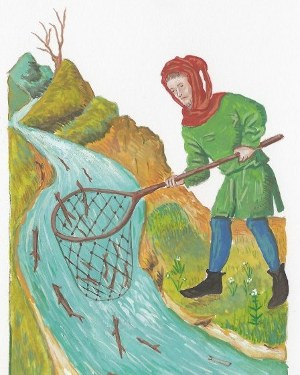
\includegraphics{../media/sample_game_cover.jpg} \end{center} 

\begin{itemize}
\item Read the \textbf{\href{\#instructions}{instructions}} or start the game \textbf{\href{\#1}{1}}
\end{itemize}

\hypertarget{1}{}
\pagebreak[\PAGExBREAKxPOLICY]
\textbf{\subsection*{\begin{center}\Huge{1}\end{center}}\vskip-2em}

This is the first chapter of your story.\footnote{It will present various ways to use txt2tags and textallion to create CYOA (choose your own adventure). Check the source code of this sample, and read the comments about various tips for using textallion}

You are walking on the bank of a river, in a sunny autumn day. You can see a \textbf{\href{\#man}{man}} holding a landing net. Yet he's not really fishing, he's only collecting small twigs.

\begin{itemize}
\item Enter the \textbf{\href{\#forest}{forest}} nearby.
\item Explore the \textbf{\href{\#hills}{green hills}} close to the river: \textbf{\href{\#5}{5}}
\item Ask the \textbf{\href{\#man}{man}} about the \textbf{\href{\#8}{twigs}} he's getting from the river: \textbf{\href{\#8}{8}}
\end{itemize}

\hypertarget{2}{}
\pagebreak[\PAGExBREAKxPOLICY]
\textbf{\subsection*{\begin{center}\Huge{2}\end{center}}\vskip-2em}

There is nothing interesting in this chapter. In fact this is only a test chapter.

This template story is almost empty yet, but you can improve it yourself!

Lorem ipsum dolor sit amet, consectetur adipisicing elit, sed do eiusmod tempor incididunt ut labore et dolore magna aliqua. Ut enim ad minim veniam, quis nostrud exercitation ullamco laboris nisi ut aliquip ex ea commodo consequat. Duis aute irure dolor in reprehenderit in voluptate velit esse cillum dolore eu fugiat nulla pariatur. Excepteur sint occaecat cupidatat non proident, sunt in culpa qui officia deserunt mollit anim id est laborum.

\begin{itemize}
\item Go to the left, turn to \textbf{\href{\#7}{7}}
\item Go to the right, turn to \textbf{\href{\#5}{5}}
\item Use the boat : \textbf{\href{\#7}{7}}. It could be a good solution.
\end{itemize}

\hypertarget{3}{}
\pagebreak[\PAGExBREAKxPOLICY]
\textbf{\subsection*{\begin{center}\Huge{3}\end{center}}\vskip-2em}

You are at the edge of the old forest. 

\setlength{\intextsep}{3mm} \begin{wrapfigure}{l}{0\textwidth} 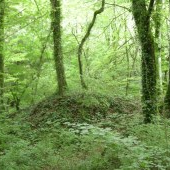
\includegraphics{../media/sample_forest.png}   \end{wrapfigure}

This forest is huge and you may get lost, so you'd better go back to the road.

\begin{itemize}
\item Go to the cliff: \textbf{\href{\#6}{6}}
\item Go back to the hills close to the beach: \textbf{\href{\#5}{5}}
\item Enter the \textbf{\href{\#forest}{forest}} anyway.
\item Go to the market place in your village: \textbf{\href{\#4}{4}}
\item Enter your home \textbf{\href{\#7}{7}} or restart \textbf{\href{\#1}{1}} the game.
\end{itemize}

\hypertarget{4}{}
\pagebreak[\PAGExBREAKxPOLICY]
\textbf{\subsection*{\begin{center}\Huge{4}\end{center}}\vskip-2em}

There is no one here.

Lorem ipsum dolor sit amet, consectetur adipisicing elit, sed do eiusmod tempor incididunt ut labore et dolore magna aliqua. Ut enim ad minim veniam, quis nostrud exercitation ullamco laboris nisi ut aliquip ex ea commodo consequat. Duis aute irure dolor in reprehenderit in voluptate velit esse cillum dolore eu fugiat nulla pariatur. Excepteur sint occaecat cupidatat non proident, sunt in culpa qui officia deserunt mollit anim id est laborum.

\begin{itemize}
\item Go up to the cliff: \textbf{\href{\#6}{6}}
\item Go to the hills: \textbf{\href{\#5}{5}}
\item Go back to the entrance of the \textbf{\href{\#village}{village}}, where you have a friend.
\end{itemize}

\hypertarget{5}{}
\pagebreak[\PAGExBREAKxPOLICY]
\textbf{\subsection*{\begin{center}\Huge{5}\end{center}}\vskip-2em}

You see nothing really interesting in the hills. There is the sea on the west and a boat on the east, not far from the \textbf{\href{\#man}{old man}} which is collecting \textbf{\href{\#8}{twigs}}.

\begin{itemize}
\item Go close to the cliff to examine the sea from above: \textbf{\href{\#6}{6}}
\item Go to the forest nearby: \textbf{\href{\#3}{3}}
\item Look inside the boat: \textbf{\href{\#2}{2}}
\item Talk to the man: \textbf{\href{\#8}{8}}
\item You decide you feel bored and go back to your home \textbf{\href{\#7}{7}} or restart \textbf{\href{\#1}{1}} the game.
\end{itemize}

\hypertarget{6}{}
\pagebreak[\PAGExBREAKxPOLICY]
\textbf{\subsection*{\begin{center}\Huge{6}\end{center}}\vskip-2em}

You stand on the edge of a cliff.\footnote{(it's very huge!)}

Lorem ipsum dolor sit amet, consectetur adipisicing elit, sed do eiusmod tempor incididunt ut labore et dolore magna aliqua. Ut enim ad minim veniam, quis nostrud exercitation ullamco laboris nisi ut aliquip ex ea commodo consequat. Duis aute irure dolor in reprehenderit in voluptate velit esse cillum dolore eu fugiat nulla pariatur. Excepteur sint occaecat cupidatat non proident, sunt in culpa qui officia deserunt mollit anim id est laborum.

Lorem ipsum dolor sit amet, consectetur adipisicing elit, sed do eiusmod tempor incididunt ut labore et dolore magna aliqua. Ut enim ad minim veniam, quis nostrud exercitation ullamco laboris nisi ut aliquip ex ea commodo consequat. Duis aute irure dolor in reprehenderit in voluptate velit esse cillum dolore eu fugiat nulla pariatur. Excepteur sint occaecat cupidatat non proident, sunt in culpa qui officia deserunt mollit anim id est laborum.

Lorem ipsum dolor sit amet, consectetur adipisicing elit, sed do eiusmod tempor incididunt ut labore et dolore magna aliqua. Ut enim ad minim veniam, quis nostrud exercitation ullamco laboris nisi ut aliquip ex ea commodo consequat. Duis aute irure dolor in reprehenderit in voluptate velit esse cillum dolore eu fugiat nulla pariatur. Excepteur sint occaecat cupidatat non proident, sunt in culpa qui officia deserunt mollit anim id est laborum.

\begin{itemize}
\item Go to the beach : \textbf{\href{\#5}{5}}
\item Go to the \textbf{\href{\#village}{village}} nearby
\end{itemize}

\hypertarget{7}{}
\pagebreak[\PAGExBREAKxPOLICY]
\textbf{\subsection*{\begin{center}\Huge{7}\end{center}}\vskip-2em}

Your home is a simple hut in the village of Uldirir.

\begin{itemize}
\item Here you can choose to continue the game by going again by the seaside, to the hills: \textbf{\href{\#5}{5}}
\item Or \textbf{\href{\#test}{test}} various things in this game.
\end{itemize}

\hypertarget{8}{}
\pagebreak[\PAGExBREAKxPOLICY]
\textbf{\subsection*{\begin{center}\Huge{8}\end{center}}\vskip-2em}

The man tells you that an extraordinary tree is growing several miles above, along the river. He's so old he cannot travel there alone. 

\begin{itemize}
\item You propose to go there for him: \textbf{\href{\#10}{10}}
\end{itemize}

\hypertarget{9}{}
\pagebreak[\PAGExBREAKxPOLICY]
\textbf{\subsection*{\begin{center}\Huge{9}\end{center}}\vskip-2em}

Nothing here yet!

\begin{itemize}
\item Restart the \textbf{\href{\#game}{game}}: \textbf{\href{\#1}{1}}
\item \textbf{\href{\#1}{1}} 

==10==[10]

Nothing here yet!
\end{itemize}

\hypertarget{game}{}
\pagebreak[\PAGExBREAKxPOLICY]
\chapter{game}

This chapter is linked from a pure keyword 

\begin{itemize}
\item Now restart the game: \textbf{\href{\#1}{1}}
\end{itemize}

\hypertarget{village}{}
\pagebreak[\PAGExBREAKxPOLICY]
\chapter{village}

\setlength{\intextsep}{3mm} \begin{wrapfigure}{l}{0\textwidth} 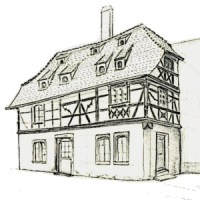
\includegraphics{../media/sample_village.png}   \end{wrapfigure}

You have a friend in the village.

\begin{itemize}
\item go to the forest: \textbf{\href{\#3}{3}}
\end{itemize}

\hypertarget{forest}{}
\pagebreak[\PAGExBREAKxPOLICY]
\chapter{forest}

As soon as you enter the forest, you hear some strange noises.

\begin{itemize}
\item Go deeper in your exploration of the \textbf{\href{\#forest\_ref\_01}{dark forest}}, or return to the \textbf{\href{\#village}{village}}.
\end{itemize}

\hypertarget{hills}{}
\pagebreak[\PAGExBREAKxPOLICY]
\chapter{hills}

blabla 

\begin{itemize}
\item go to \textbf{\href{\#5}{5}}
\end{itemize}

\hypertarget{forest_ref_01}{}
\pagebreak[\PAGExBREAKxPOLICY]
\chapter{forest\_ref\_01}

This part is deeper in the \textbf{\href{\#forest}{forest}}.

\begin{itemize}
\item Restart the game \textbf{\href{\#1}{1}}
\end{itemize}

\hypertarget{man}{}
\pagebreak[\PAGExBREAKxPOLICY]
\chapter{man}

The man has a long beard and some strange nostrils. He's quite aged and looks quite crazy.

\begin{itemize}
\item Talk to the man: \textbf{\href{\#8}{8}}
\item Go back home: \textbf{\href{\#7}{7}}
\end{itemize}

\hypertarget{test}{}
\pagebreak[\PAGExBREAKxPOLICY]
\chapter{test}

This part is for testing purpose only.

\begin{itemize}
\item Secret chapter: turn to \textbf{\href{\#2}{2}}

\item \textbf{\href{\#village}{tiny village}} 
\item \textbf{\href{\#village}{tiny village}}.
\item \textbf{\href{\#village}{tiny village}}
\item this \textbf{\href{\#village}{village}}, nearby, \textbf{\href{\#village}{tiny village}}.

\item Enter your home \textbf{\href{\#7}{7}} or restart \textbf{\href{\#1}{1}} the game.
\item Enter your home \textbf{\href{\#7}{7}} or restart \textbf{\href{\#1}{1}} the game.
\item go deeper in the \textbf{\href{\#forest\_ref\_01}{dark forest}}, check \textbf{\href{\#game}{this game info}} or return to \textbf{\href{\#village}{village}}
\end{itemize}

You see nothing really interesting in the hills. There is the sea on the west and a boat on the east, not far from the \textbf{\href{\#man}{old man}} which is collecting \textbf{\href{\#8}{twigs}}.

You see nothing really interesting in the hills. There is the sea on the west and a boat on the east, not far from the \textbf{\href{\#man}{old man}} which is collecting \textbf{\href{\#8}{twigs}}.

\hypertarget{instructions}{}
\pagebreak[\PAGExBREAKxPOLICY]
\chapter{instructions}

Lorem ipsum dolor sit amet, consectetur adipisicing elit, sed do eiusmod tempor incididunt ut labore et dolore magna aliqua. Ut enim ad minim veniam, quis nostrud exercitation ullamco laboris nisi ut aliquip ex ea commodo consequat. Duis aute irure dolor in reprehenderit in voluptate velit esse cillum dolore eu fugiat nulla pariatur. Excepteur sint occaecat cupidatat non proident, sunt in culpa qui officia deserunt mollit anim id est laborum.

% LaTeX2e code generated by txt2tags 2.6. (http://txt2tags.org)
% cmdline: txt2tags -T ..//templates/latex.tex --config-file ..//core/txt2cyoa.t2t -t tex --no-toc --outfile sample_cyoa.tex sample_cyoa.t2t

\end{LARGE}
\end{document}
